\chapter{System Architecture and Development} \label{sec:systemdevelopment}

In the previous chapter I presented the requirements the solution had to achieve and evaluated different development options, discussing their advantages and disadvantages.
I closed the chapter with a solution proposition, where I justified hardware and software choices.
In this chapter I will present the implementation of such solution, going through the architecture design, configuration and development. 

\section{Architecture}

The architecture identically follows the EPCGlobal example, presented in figure~\ref{fig:archstructure} on chapter~\ref{sec:epcglobal}.
A detailed overview of the architecture is illustrated in figure~\ref{fig:practicalarchitecture}.

\begin{figure}
    \centering
    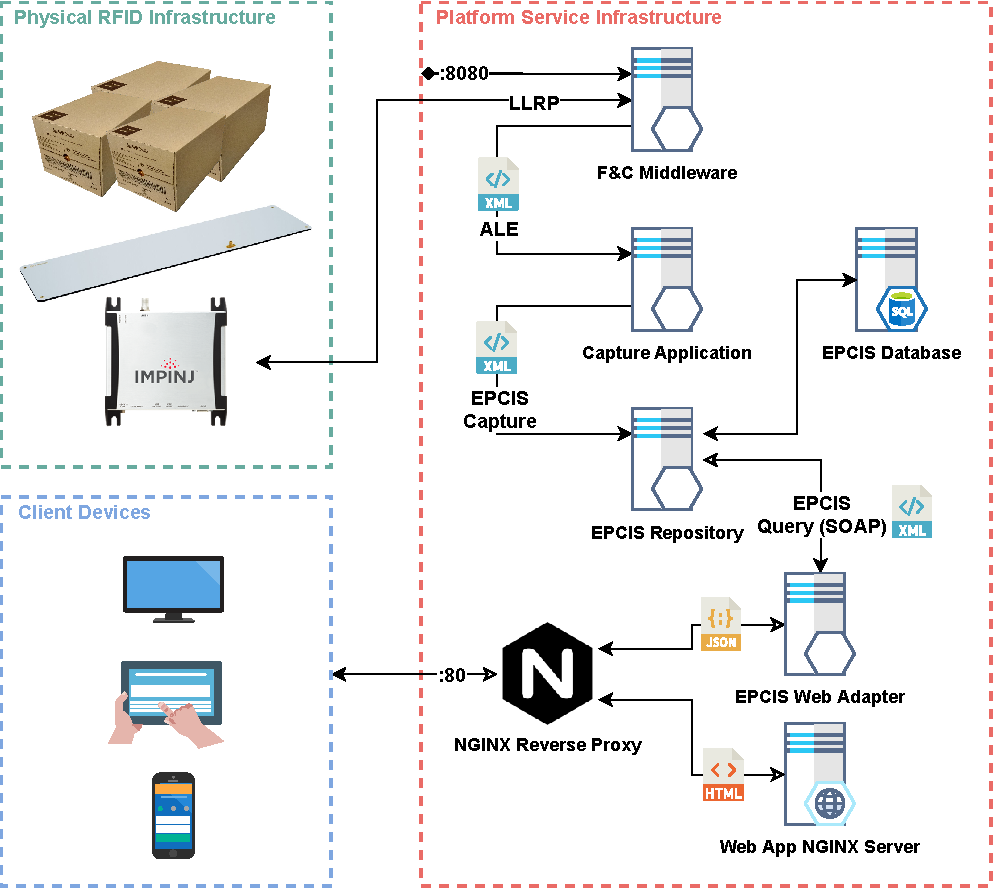
\includegraphics[width=\textwidth]{figs/platform_diagram.pdf}
    \caption{Overview of the solution architecture developed in this dissertation} 
    \label{fig:practicalarchitecture}
\end{figure}

The Impinj Speedway R120 reader and Keonn Advantenna-p14 are attached behind the bottom shelf, as shown in figure~\ref{fig:shelvephoto}, radiating the entire shelve.
The reader interrogates the tags, using the \ac{gen2} Tag Air Standard, following the active \acp{rospec} configured prior to the inventory.
The inventory information is sent inside \texttt{RO\_ACCESS\_REPORT} messages, to the \ac{llrp} interface of the middleware.

\begin{figure}
    \centering
    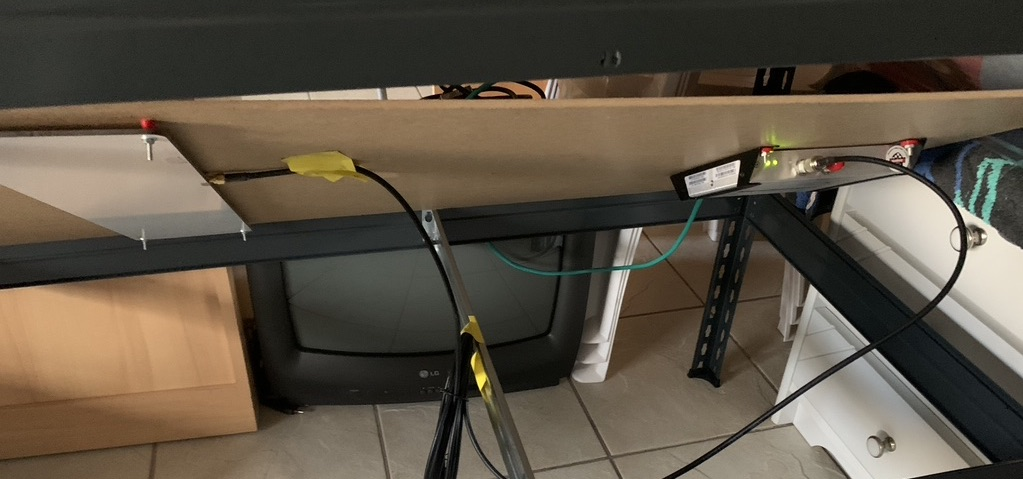
\includegraphics[width=\textwidth]{figs/completeshelve_photo.jpeg}
    \caption{Photograph of the Keonn Advantenna-p14 and Impinj Speedway R120 attached behind the bottom shelf}
    \label{fig:shelvephoto}
\end{figure}

The Fosstrak \ac{fc} middlware receives the inventory information from the reader, processes it, following the configured \acp{ecspec}, and periodically generates \acp{ecreport}, which are sent to the capture application \ac{ale} capture interface.

The Fosstrak capture application receives the \acp{ecreport}, contextualizes them and runs additional business logic. The contextualized data is aggregated in \acs{epcis} event documents, following the \ac{cbv} vocabulary guidelines, and sent to the \ac{epcis} repository.

The \ac{epcis} repository permanently saves the \ac{epcis} data in to the \ac{epcis} database. The \ac{epcis} repository exposes the \ac{soap} query interface, which can be used to retrieve information.

The managing application to visualize the smart shelve inventory, was made using web technologies. The application is served to browsers by an NGINX static file server. The browser running the application queries the data in the \ac{epcis} repository.
Modern browsers do not support \ac{soap} natively. 
To mitigate this problem, the requests pass through a crude \ac{epcis} web adapter, serving as a proxy between web applications and the \ac{epcis} repository. 
The proxy adapts the \ac{soap} \ac{xml} requests into \ac{http} and \ac{json} endpoints, which modern browsers understand.

All client requests hitting the platform go through an NGINX reverse proxy. This hides the topology and characteristics of the back-end servers, removing the direct internet access to them. The services on the platform are kept inside a non-public subnet and concentrate the access control on that single point. The NGINX server also allows load balancing between the services, which is useful when there is a need to scale the platform. The proxy also deals with cross-origin resource sharing mechanism, freeing the servers from dealing with it.

All services in the platform infrastructure are containerized using Docker, and orchestrated using Docker Compose. The yaml compose file, containing the description of  can be consulted in appendix~\ref{apx:composefile}.
All the code, configurations, dockerfiles and such can be consulted in the Github dissertation repository at \url{https://github.com/dvcorreia/epc-smart-shelve}~\cite{DvcorreiaEpcsmartshelve}.

\section{\acs{epc} Serialization Plan}

When companies adhere to the EPCGlobal framework, there are a few things that have to be deliberated.
One of those is delineating the \acs{epc} serialization plan, where an evaluation of unique products and serial numbers is made.
The plan has to ensure that a company has enough unique product numbers to identify current and future products.

In the case of this dissertation, the serialization plan was already performed by Nespresso.
Each of their products has already an assigned \ac{gtin}, including the cardboard case for transport.

From the product cases for transport are identified by the GS1-$128$ barcode, and sleeves by \acs{ean}-$13$ barcode. From those used for testing, two Nespresso company prefixes were present: $76300544$ and $76300396$ respectively. Nestlé Nespresso SA has many more registered. Searching in GS1 Company Database (GEPIR), I found $18$ more, registered in Switzerland.
From the \acs{ean}-$13$ barcode in sleeves, the \acs{gtin}-$13$ can be inferred and converted to \acs{gtin}-$14$ for \ac{sgtin}-$96$ encoding on \ac{gen2} \ac{epc} \acs{rfid} tags, which was covered in section~\ref{sec:sgtin}.
For the GS1-$128$ barcode in product cases for transport, an example of the barcode deconstruction is illustrated in figure~\ref{fig:gs1-128barcode}.

\begin{figure}
    \centering
    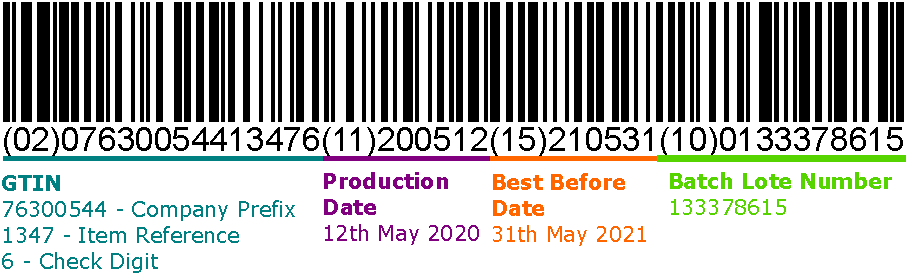
\includegraphics[width=\textwidth]{figs/gs1-128barcode.pdf}
    \caption{Deconstruction of a GS1-$128$ barcode from a Volluto coffee cardboard case for transport used in this dissertation has a test product (GS1 AI IDs on \acs{tds} Section F.1~\cite{EPCTagData})}
    \label{fig:gs1-128barcode}
\end{figure}

With the \acs{gtin}-$14$, it is possible to encode \ac{sgtin}-$96$ in \ac{gen2} tags. To write the \acp{epc} in the testing tags, it was used the Impinj Octane Java SKD \texttt{WriteEpc.java} sample code, adapted with the \ac{tdt} engine. Instead of generating a random \ac{epc}, the Fosstrak \ac{tdt} engine was used to encode a valid \ac{epc} with the correspondent company prefix, item reference and serial in to hexadecimal, which can be passed to the \texttt{TagWriteOp} class to configure the reader and program the tag.

A tag was attached to each sleeve and transport box, with their correspondent \ac{gtin} and unique serial number as a \ac{sgtin}-$96$.

\section{Reader} \label{sec:readerconfiguration}

Throughout this dissertation, the reader was configured employing three approaches: using the Impinj Octane Java SDK~\cite{OctaneSDK}, the Impinj LTK using \ac{xml} configuration files~\cite{LTKXMLJava} and with Fosstrak \ac{llrp}Comander client software~\cite{FosstrakLLRPCommander}.
Each one has their advantages and disadvantages.

In section~\ref{sec:llrp}, I mentioned that \ac{xml} is used to provide a human readable and abstract the \ac{llrp} standard.
In fact, it can be used to describe messages like the \textit{ADD\_ROSPEC} and \textit{SET\_READER\_CONFIG}.
This makes it easy to create and manage configuration files compared to code, which requires knowledge of each reader manufactured SDK and referent programming language, to to maintain.

When configuring the reader with the \acs{llrp}Commander or LTK-\ac{xml}, the configurations can be interchangeable, sharing the same \ac{xml} file. These methods have a few flaws. From what I experienced, \ac{llrp}Commander has some problems dealing with Impinj extensions and filter parameters, and requires Eclipse $3.3$ 2007 build, which is old and not maintained.
The Impinj LTK-\ac{xml} configuration method also seems to have some problems dealing with Impinj extensions~\footnote{Example: specifying \texttt{ImpinjInventorySearchMode} returns unable to convert LTK-XML to Internal Object. \texttt{C1G2InventoryCommand} has unknown element \texttt{ImpinjInventorySearchMode} which exists and is documented~\cite{ImpinjLTKProgrammers}}.
Other problem is the \ac{xml} parser which seems to require fields, ignored Impinj reader in certain conditions, which have to be present in order to validate de \ac{xsd} schema for the configuration to be validated (e.g\ \texttt{TagInventoryStateAware}, \texttt{Tari}).

The suggested approach is using the Octane SKD. It forfeits the advantages of a \ac{xml} configuration file, but it provides all the features expected from the reader, and is reliable and fast to configure.
Octane 6.2.0, last version at the time of this dissertation, is based on \ac{llrp} version 1.0.1, which does not support some Class 1 \ac{gen2} version 1.2.0 features natively in the \ac{llrp} LTK implementation~\cite{ImpinjOctaneLLRP}. Octane includes vendor extensions in the SDK to expose the underlying air protocol features.
The reader firmware used was version 5.12.2.240 (Build cbc9ad1d0d1).

The full code used to configure the reader can be consulted in appendix~\ref{apx:octanereaderconfig}.
The \ac{xml} configuration files used with \ac{llrp}Commander and LTK-\acs{xml} program can be consulted in appendix~\ref{apx:xmlreaderconfig}.
The parameters configuration will be discussed in the next section.

\subsection{Antenna and \acs{gen2} Settings}

In section~\ref{sec:llrpspecs} I presented the \ac{rospec} used to control the reader operation through the \ac{llrp} protocol. The \ac{rospec} defined for this solution will be discussed in detail in this section.
Use appendix~\ref{apx:xmlreaderconfig} \ac{xml} configuration files as reference.

It is good practice in \ac{uhf} \ac{rfid} systems to configure antennas aside from the \ac{rospec} definition. \ac{rf} antenna parameters are dependent on \ac{rfid} hardware and environment in which the system is deployed. \acp{rospec} allow antenna configuration, but should only specify reader control operation, namely inventory logic operations. This ensures configuration interoperability between same logic deployments in disparate \ac{rf} environments.

\subsubsection{Power}

To do so, \ac{llrp} defines the \textit{SET\_READER\_CONFIG} message with the \texttt{AntennaConfiguration} parameter.
This parameter contains a few important parameters and fields:

\texttt{ReceiverSensitivity} specifies the effective receive sensitivity level in dBm. While testing the solution, the \ac{rf} environment conditions were optimal, which allowed setting the reader to the maximum sensitivity of $-80$dBm. This sensitivity is index $1$ on the \texttt{ReceiveSensitivityTableEntry}. For the R120 reader capabilities consult appendix~\ref{apx:readercapabilities}.
\texttt{TransmitPower} specifies the transmission power provided to the antennas as an offset into the \texttt{TransmitPowerLevelTableEntry}. For the Speedway R120 reader power with PoE, the maximum transmission power is $30$ dBm, which is index of $81$, used in this dissertation tests~\cite{ImpinjOctaneLLRP, SettingReceiveSensitivity}.

\subsubsection{Class 1 \ac{gen2} Settings}

The \texttt{C1G2InventoryCommand} parameter is were the Class 1 \ac{gen2} air protocol is tunned.
\texttt{TagInventoryStateAware} flag is used to determine how to process all the \texttt{C1G2Filter} and \texttt{C1G2Singulation} parameters in this command~\footnote{At a functional level, if the Client is managing the tag states during an inventory operation (i.e\ the Client is specifying Class1 \ac{gen2} tag Select command Target and Action values), then it will set that flag to true and pass the appropriate fields in the C1G2 Filter and C1G2 Singulation parameters. If a reader set \texttt{CanDoTagInventoryStateAwareSingulation} to False in LLRPCapabilities, then the Reader shall ignore the \texttt{TagInventoryStateAware} flag~\cite{LowLevelReader}}.

The \texttt{C1G2RFControl} parameter specifies Speedway Gen2 modes selected by Impinj system engineering to provide the best performance. No Tari adjustment is necessary. Tari values passed by the client will be ignored~\cite{ImpinjOctaneLLRP}.

\texttt{ModeIndex} selects the operation mode~\cite{ReaderModesMade, ImpinjOctaneLLRP}. For the use case of this dissertation, it can be one of the three bellow, depending on the \ac{rf} environment in which the system is deployed: 

\begin{itemize}
    \item $1002$ (AutoSet Dense Reader Deep Scan) configures the Reader to choose the best \ac{gen2} link parameters for the environments where the tag population is relatively static and we wish to attempt to search for the weakest tag~\cite{ReaderMode1002};
    \item $1003$ (Autoset Static Fast) is an adaptation of Autoset Dense Reader Deep Scan for good \ac{rf} environments;
    \item $1004$ (AutoSet Static Dense Reader) is an adaptation of Autoset Dense Reader Deep Scan for difficult \ac{rf} environments.
\end{itemize}

The option used was \texttt{ModeIndex} $1002$. The $1004$ is not currently available for the R120 in the ETSI european \ac{uhf} band. The $1003$ does not provide confidence in warehouse malls, where other readers systems can operate and create poor \ac{rf} environment conditions.

\subsubsection{Singulation Configuration}

Impinj offers a few custom parameters supported in Octane \ac{llrp}, namely the \texttt{ImpinjInventorySearchMode}, a Impinj-specific inventory search mode. 
To understand search modes, we have to understand sessions. This thematic goes deep in to the \ac{gen2} air protocol and will only briefly contextualized. \ac{gen2} defines up to four tag sessions. Sessions are states tags can transit to, in order to help the reader attempt to singulate, i.g\ read, tags.
Sessions can be used to determine when a tag will respond to a query from the reader, and/or allow tags to maintain independent states when communicating with multiple readers at the same time. 

Impinj readers implement state unaware singulation, in that they provide a high-level control over the search algorithm, through \texttt{ImpinjInventorySearchMode} parameter, not interfering with any of the standard \ac{llrp}/\ac{gen2} settings~\cite{ImpinjOctaneLLRP, UnderstandingEPCGen2}.
Impinj search modes can be consulted in appendix~\ref{apx:searchmodes}.
In this dissertation we used Tag Focus to make sure every tag was read. This was possible only because we used HID 6H2E43 tags with use Monza chips in this dissertation. For generic tags I recommend using Dual Target Inventory search mode.

Using purely \ac{llrp} settings for configuration interchangeability with other reader manufacturers, \ac{gen2} provides the \texttt{C1G2SingulationControl} to control the singulation process in the Class 1 \ac{gen2} air protocol:

\begin{itemize}
    \item \texttt{TagTransitTime}: This is the measure of expected tag mobility in the field of view of the antenna where this inventory operation is getting executed.
    \item \texttt{TagPopulation}: This is the expected tag population in the field of view of the antenna.
    \item Session ID: This is the C1G2 session number that the tags use to update the inventory state upon successful singulation.
    \item \texttt{TagInventoryStateAwareSingulationAction}: used if the \texttt{TagInventoryStateAware} flag is set to true in the \texttt{InventoryParameterSpec}. It is used to query, select and deselect target tag population in the a selected session.
\end{itemize}

Configurations with tunning of these setting were done for testing, but were not used in the final prototype presented in this dissertation, so no further detail will be done.

\subsubsection{\ac{gen2} \ac{epc} Filtering}

In the \ac{llrp} and LTK-\ac{xml} configurations I could not make it work, but in the Java Octane reader configuration, used to configure the reader in the shelve solution, it was possible to implement \ac{epc} filtering directly through the Class 1 \ac{gen2} protocol.

The filtering works by defining a mask, which is sent in the air protocol in the query process, for tags to evaluate if they correspond to the desired population to be inventoried. Only tags corresponding to such filter answer back.
The \ac{c1g2} filter can be used to match any \ac{gen2} tag memory data, not \ac{epc} exclusively.
Air protocol filtering greatly reduces tag-to-tag interference, decreases environment \ac{rf} noise, lowers networking traffic in pin-point singulation inventories, and removes filtering work otherwise made by the middleware.

The \ac{c1g2} protocol provides tree parameters which can be used to specify the filter: 

\begin{itemize}
  \item \texttt{setBitPointer} (integer): corresponds to the start bit position to apply the tag mask when performing tag filtering;
  \item \texttt{setBitCount} (integer): defines the number of bits to compare against the mask, starting with the bit pointer;
  \item \texttt{mask}: is the mask to be compared. It must be of a bit length divisible by $8$, begin usually defined in hexadecimal~\cite{LowLevelReader}.
\end{itemize}

In figure~\ref{fig:c1g2filter} It can be observed a deduction of the parameters presented previously.
To match to both company prefixes found in the test products, the bit pointer should point to the first bit of the company prefix, which will be the pointer to the \ac{epc} memory plus $14$ bits.
The bit count should be the size of the company prefix, $27$ bits. The mask has to be at least $32$ bits, which for company prefix of ``$76300544$'' the mask could be \texttt{91882001} and for ``$76300396$'' \texttt{91880D82}.

\begin{figure}
  \centering
  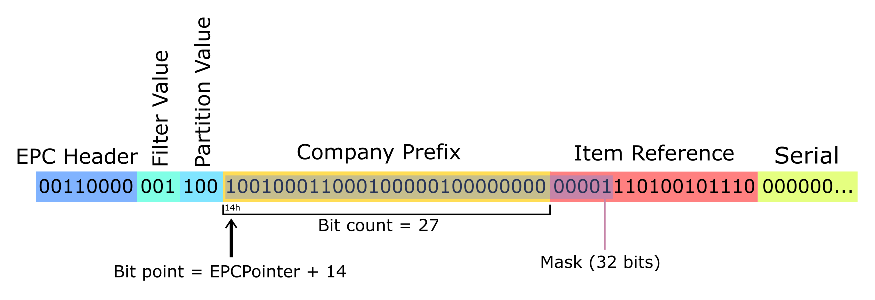
\includegraphics[width=\textwidth]{figs/c1g2filter.eps}
  \caption{Illustration of company prefix \ac{c1g2} filtering parameter deduction}
  \label{fig:c1g2filter}
\end{figure}

\subsection{Operation Configuration}

With the antenna and \ac{gen2} protocol configured, we can focus on the operations the reader has no perform on the tag population.

In this dissertation we want to perform an inventory of the products stored in the shelve. Reader inventory operations are described in a \ac{rospec}.
In section~\ref{sec:llrpspecs}, I described the parameters composing an \ac{rospec} document. Particularly, the \texttt{ROBoundarySpec}, \texttt{\acs{aispec}} and \texttt{ROReportSpec} are interesting to be discussed.

\subsubsection{ROBoundarySpec}

The \texttt{ROBoundarySpec} parameter describes the lifetime of the Reader inventory and survey operations.
The lifetime can be configured in different ways, with no clear superior choice, being to the integrator engineer sensibility to project and evaluate an effective \ac{spec}.

In designing this \ac{spec} solution, the configuration made previously, regarding the search singulation algorithm mode, had to be accounted.
For the Tag Focus search mode, the reader inventories tags in state A, transitioning the tags to state B upon singulation. Tags transition back to state A in less than $5$ seconds, when de-energized~\cite{ImpinjOctaneLLRP}.
Dual Target search mode inventories tags in state A, transitioning the tags to state B. Them inventories tags in state B, transitioning the tags back to state A.
Evaluating both search modes, the solution used consisted in periodically inventor the tags, every $5$ seconds with a $2$ seconds inventory exercitation time~\cite{ImpinjOctaneLLRP, UnderstandingEPCGen2}.
This allowed a full Tag Focus search inventory search cycle while providing enough time for the Dual Target search mode.

Translating the lifetime plan to the \ac{spec} parameters, it should look like code~\ref{code:boudaryspec}. The \texttt{ROSpecStartTrigger} should be periodic, with a period of $5000$ milliseconds, and no offset. The \texttt{ROSpecStopTrigger} triggers $2000$ milliseconds after receiving the trigger to start the \ac{rospec}. 

\begin{listing}
    \begin{minted}[linenos]{xml}
    <ROBoundarySpec>
      <ROSpecStartTrigger>
        <ROSpecStartTriggerType>Periodic<ROSpecStartTriggerType>
        <PeriodicTriggerValue>
          <Offset>0</Offset>
          <Period>5000</Period>
        </PeriodicTriggerValue>
      </ROSpecStartTrigger>
      <ROSpecStopTrigger>
        <ROSpecStopTriggerType>Duration<ROSpecStopTriggerType>
        <DurationTriggerValue>2000</DurationTriggerValue>
      </ROSpecStopTrigger>
    </ROBoundarySpec>
    \end{minted}
    \caption{}
    \label{code:boudaryspec}
\end{listing}

\subsubsection{\acl{aispec}}

For the \ac{aispec} parameters, most of the configuration was already done in through the \textit{SET\_READER\_CONFIG} message, presented in the previous section.

It is important to specify the air protocol, namely EPCGlobalClass1Gen2, inside the \texttt{InventoryParameterSpec}.
The \texttt{AISpecStopTrigger} parameter defines the terminating boundary of an antenna inventory operation~\cite{LowLevelReader}, which was set to Null to stop when \ac{rospec} is terminated.

\subsubsection{Report Operation Report Spec (ROReportSpec)}

The \texttt{ROReportSpec} parameter describes the messages and parameters used in reports, event notifications and keepalives that are generated by the Reader and sent to the Client.

Important to consider, evaluating systems, is when reports are generated and sent to the Client. 
In the use case in this dissertation we are not concerned with near real-time updates on the state of the inventory. We are interested in the networking infrastructure in which the system is deployed. In mall warehouses, this infrastructure is most likely shared with other companies. The traffic generated by readers should be controlled to not overburden the network.

With that in mind, the report generation is triggered by the end of the \ac{rospec}. This will generate a report periodically every $5$ seconds.
For this behavior \texttt{ROReportTrigger} should be set to \texttt{Upon\_N\_Tags\_Or\_End\_Of\_ROSpec} with N$=0$, meaning unlimited tag in the field of view of the antenna~\cite{LowLevelReader}.

The \texttt{ROReportSpec} also selects which content the report sent to the client should include.
The \ac{epc} is always delivered by default.
In terms of the content useful to retrieve from the reader inventory singulation, the \texttt{ROSpecID}, \texttt{FirstSeenTimestamp} and \texttt{LastSeenTimestamp} are in the interests of the application. 
This content allows the middleware to generated accurate tag time information without real-time report delivery, which will be discussed next.

\section{\acs{fc} Middleware}

To configure de Fosstrak \ac{fc} middleware we need to define \acp{lrspec} and \acp{ecspec}.
\acp{lrspec} must identify the reader, its \ac{ip} address, port and type, for abstraction layers required in some proprietary reader communication interfaces.
For the Impinj Speedway R120, using the \ac{llrp} interface, the configuration can be seen in code~\ref{code:lrspec}.

Following the requirements of the solution, the configuration of the \ac{ecspec} has to provide $2$ \acp{ecreport} to the capture application: one for informing the tag \acp{uri} added to the shelve and another informing tag \ac{uri} removed from the shelve.
The configuration can be seen in code~\ref{code:ecspec}.
Every $5$ seconds, the middleware will report to the capture application added and removed tag \acp{uri}.
This configuration can be has complex has the integrator seems required. Since \ac{epc} filtering was achieved through the \ac{c1g2} protocol, no filtering was required in the middleware. For an example of what a more complex shelve middleware would look like for this type of application, consult appendix~\ref{apx:complexecspec}.

\section{Capture application}

The Fosstrak Capture application allows the definition of business logic through the Drools engine, a business rules management system.

For the requirements for this solutions, it were defined two rules: one for added items and another for removed items. Each generates a single \ac{epcis} ObjectEvent document following \ac{cbv} guidelines. The ObjectEvent contains:

\begin{itemize}
  \item \textbf{\ac{epc} List}: containing the tag \acp{uri}.
  \item \textbf{Action type}: \texttt{OBSERVED}.
  \item \textbf{Event time}: ISO 8601 generated automatically by the capture application software.
  \item \textbf{Event Time Zone Offset}: ISO 8601 generated automatically by the capture application software.
  \item \textbf{Read Point}: ``\texttt{urn:epc:id:sgln:76300544.00000.1}'', a fictitious read point created for test purposes. It identifies the shelve within the business location.
  \item \textbf{Business Location}: ``\texttt{urn:epc:id:sgln:76300544.00000.0}'', a fictitious business location created for test purposes. Identifies the Nespresso boutique store in Aveiro. 
  \item \textbf{Business Step}: ``\texttt{urn:epcglobal:cbv:bizstep:storing}'' for added items; ``\texttt{urn:epcglobal:cbv:bizstep:unpacking}'' for removed items. 
  \item \textbf{Disposition}: ``\texttt{urn:epcglobal:cbv:disp:sellable\_not\_accessible}'' for added items; ``\texttt{urn:epcglobal:cbv:disp:partially\_dispensed}'' for removed items.
\end{itemize}

The capture application, in a real world context, could implement much more complex business logic, to provide information to other inventory data services, process data, and present better context regarding the \ac{cbv}. 

\section{\acs{epcis} repository and Adapter}

The \ac{epcis} repository does not require any configuration, except for containerizing the service and provide a SQL database instance configured with the \ac{epcis} schema.

To facilitate the interaction with the \ac{epcis} repository by modern web browsers, an adapter service was developed in the Golang programming language. The service implements a crude and partial adapter for the \ac{epcis} Query Interface. A functional block illustration can be seen in figure~\ref{fig:epcisadapter}. It implements endpoints for the \texttt{poll} \texttt{SimpleEventQuery} and \texttt{subscribe} operations.

For the \texttt{poll} operation, the service translates \ac{http} queries in to \ac{soap} envelopes, which are sent to the \ac{epcis} repository. Response data is translated form \ac{xml} in to \ac{json} and sent back to the web client. 
For the \texttt{subscribe} operation, the subscription endpoint converts the query into \ac{soap} and registers the subscription in the \ac{epcis} repository. The event data is sent by the \ac{epcis} repository to the adapter, were is delivered in \ac{json} using websockets.
The \ac{epcis} data model in Golang used for this service can be seen in appendix~\ref{apx:epcisgolang}. The full service code can be consulted in the dissertation Github repository~\cite{DvcorreiaEpcsmartshelve}.

\begin{figure}
  \centering
  \caption{Functional block illustration of the \acs{epcis}-adapter developed in this dissertation}
  \label{fig:epcisadapter}
\end{figure}

\section{Managements application}

\begin{figure}
  \centering
  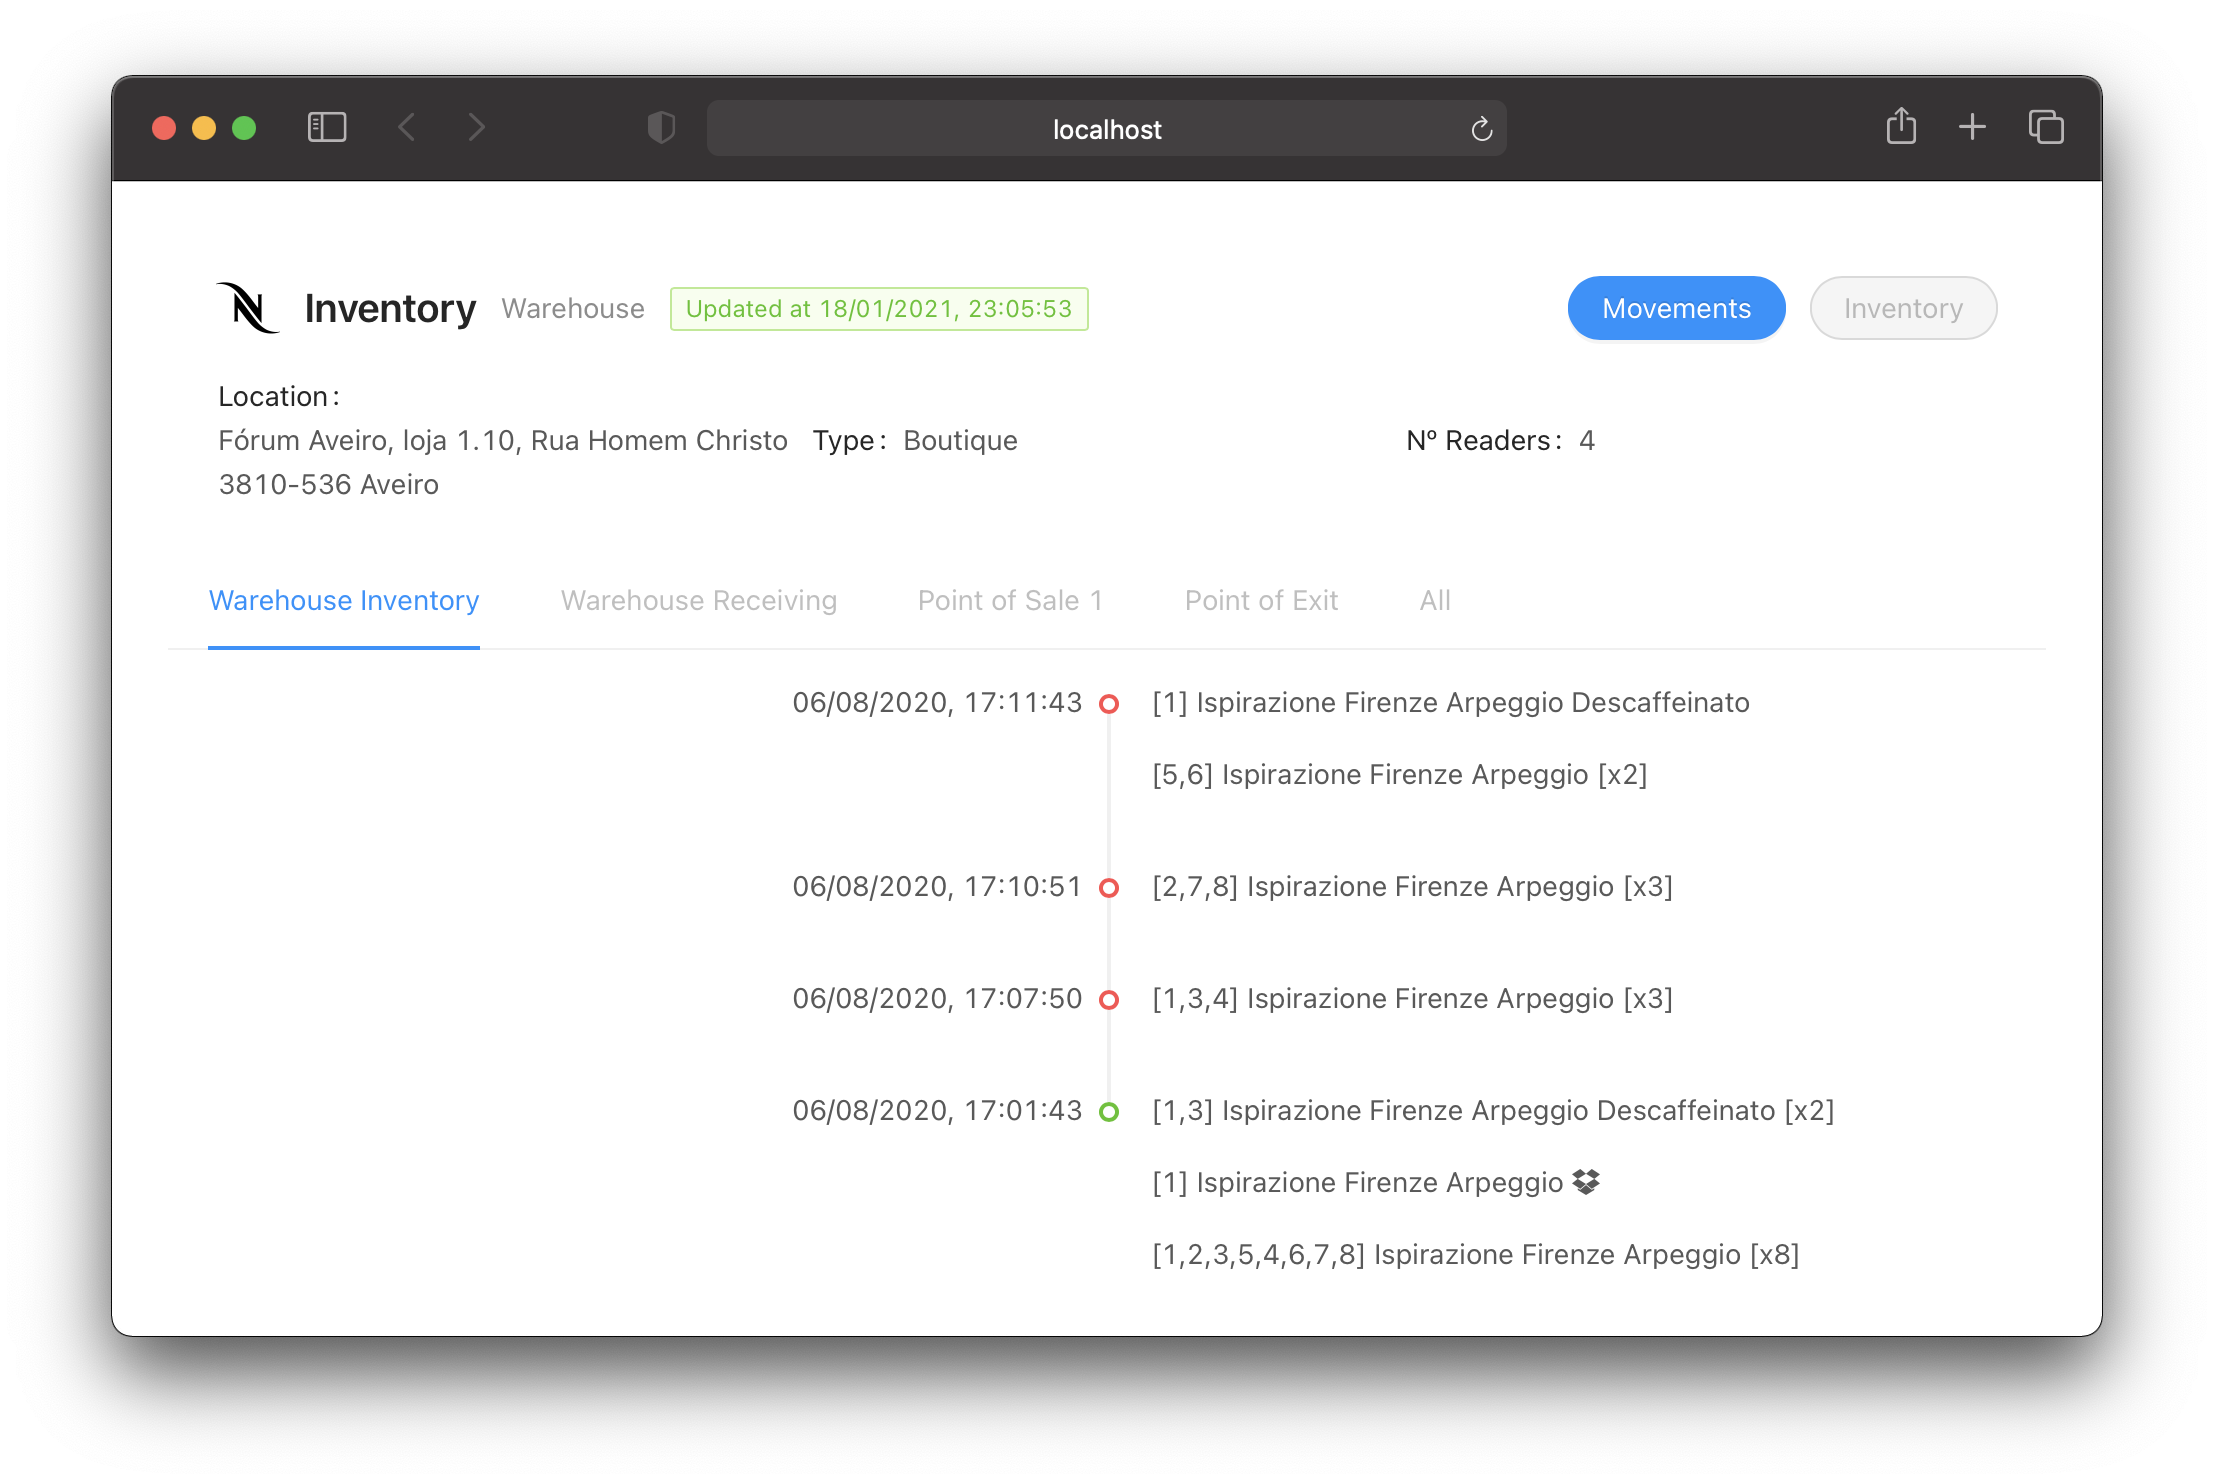
\includegraphics[width=\textwidth]{figs/webmanagement.png}
  \caption{}
  \label{fig:webinterface}
\end{figure}